\documentclass{article}

\usepackage{graphicx}
\usepackage{tikz}
\usepackage{tikzsymbols}
\usetikzlibrary{calc,patterns,shapes.geometric}
\pagestyle{empty}
\usepackage[margin=0pt]{geometry}
\geometry{papersize={14in,12in}}

\def\centerarc[#1](#2)(#3:#4:#5){\draw[#1] ($(#2)+({#5*cos(#3)},{#5*sin(#3)})$) arc (#3:#4:#5);}

\begin{document}
	\begin{figure}
		\centering
		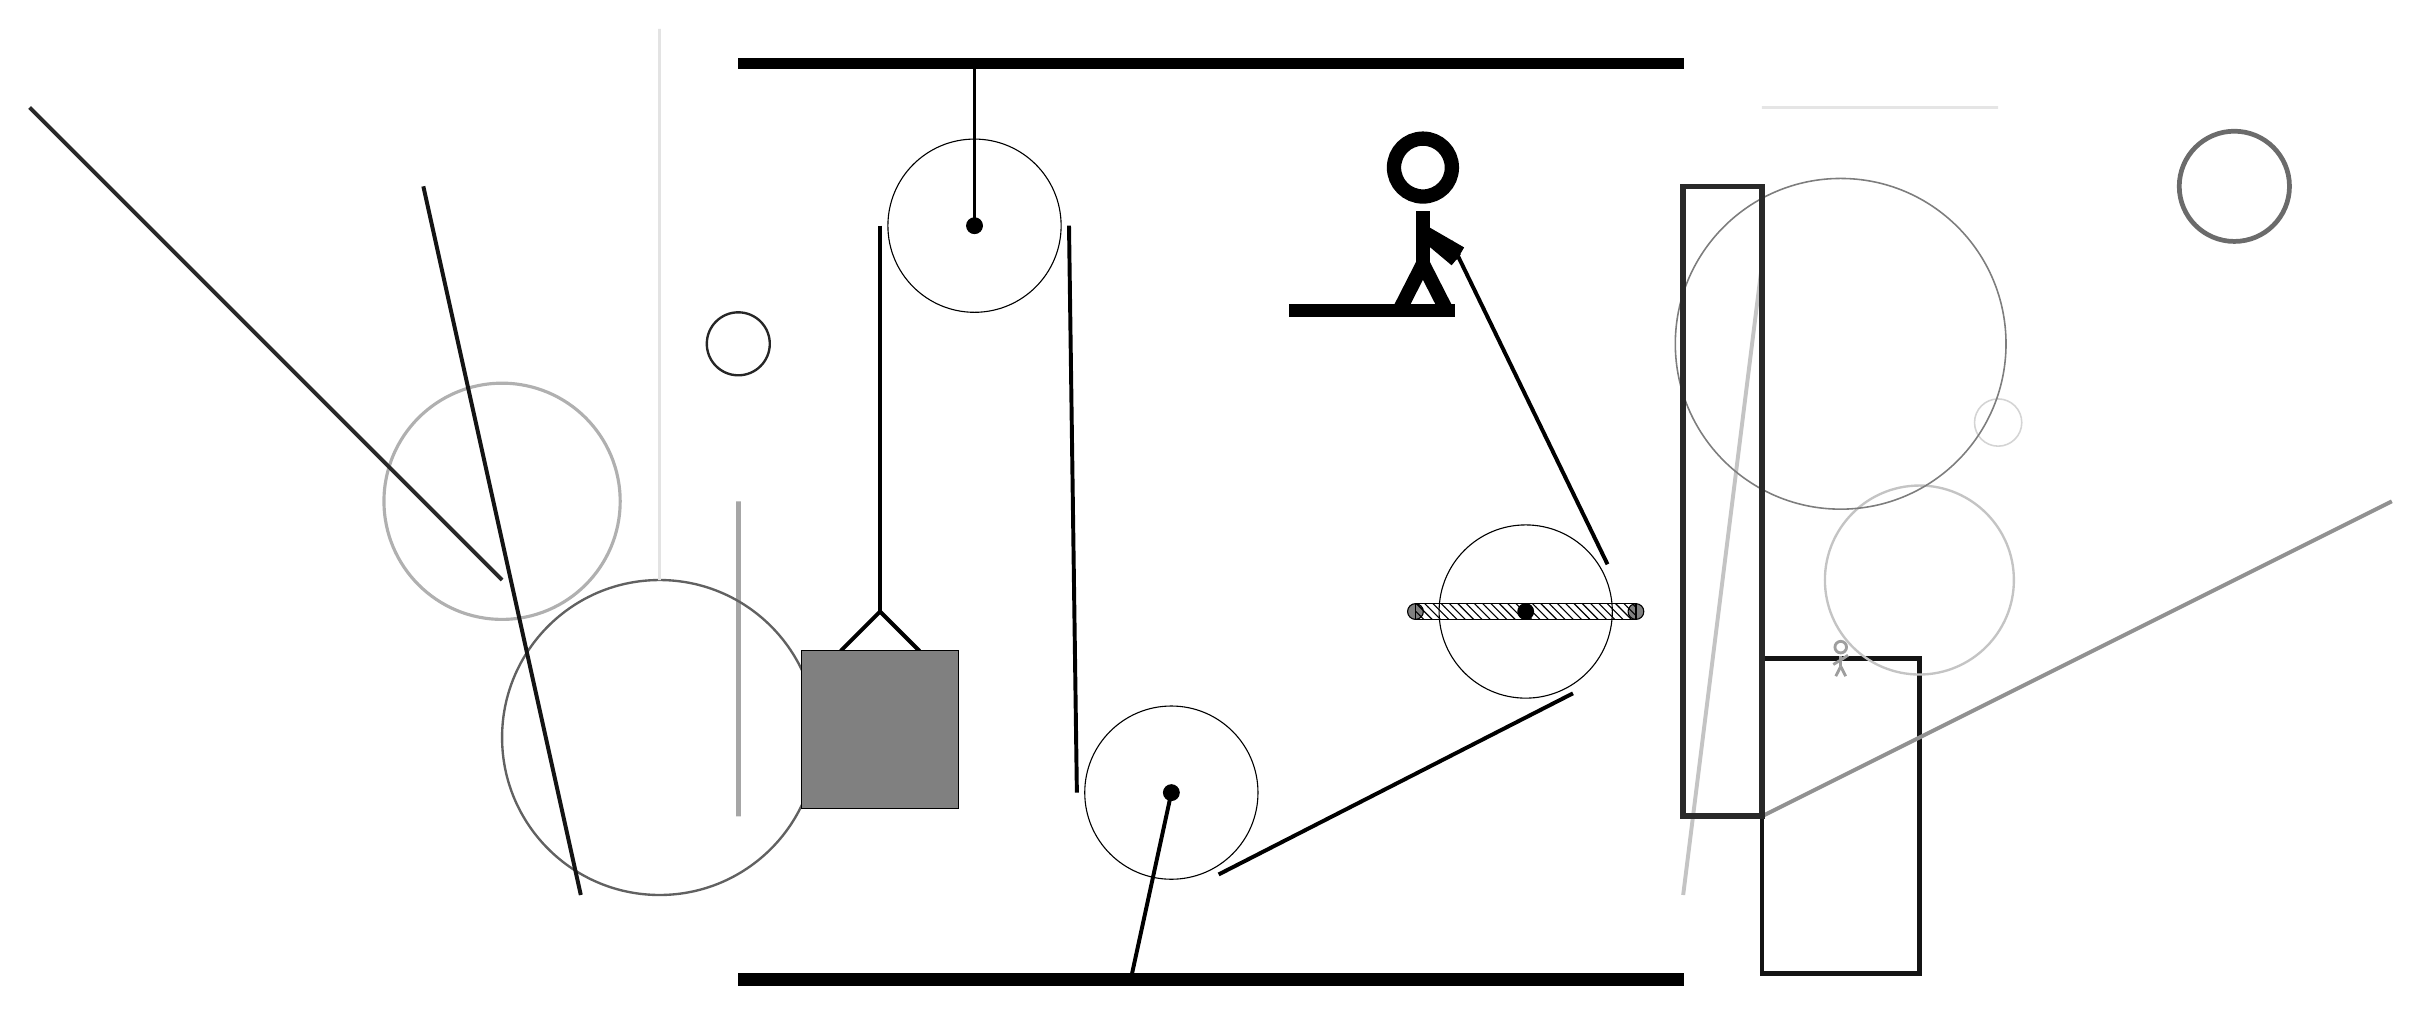
\begin{tikzpicture}
			%%%%% START %%%%%
			
			\draw[fill=black] (-2, 11.5) rectangle (10, 11.625);
			
			\draw (1, 9.5) circle (1.1);
			\draw[fill=black] (1, 9.5) circle (0.1);
			\draw[line width=0.5mm] (1, 11.5) -- (1, 9.5);
			
			\draw (3.5, 2.3) circle (1.1);
			\draw[fill=black] (3.5, 2.3) circle (0.1);
			\draw[line width=0.5mm] (3.5, 2.3) -- (3.0, 0);
			
			\draw[line width=0.6mm, color=black!92] (11, 4) rectangle (13, 0);
			
			\draw[line width=0.3mm, color=black!10] (11, 11) rectangle (14, 11);
			\draw [line width=0.3mm, color=black!85](-2, 8) circle (0.4);
			\draw[line width=0.6mm, color=black!35] (-2, 2) rectangle (-2, 6);
			\node[line width=0.2mm, color=black!38] at (12, 4) {\Strichmaxerl[2][31][33]};
			\draw [line width=0.6mm, color=black!58](17, 10) circle (0.7);
			\draw [line width=0.3mm, color=black!23](13, 5) circle (1.2);
			\draw [line width=0.4mm, color=black!31](-5, 6) circle (1.5);
			\draw[line width=0.5mm, color=black!23](11, 9) -- (10, 1);
			\draw [line width=0.2mm, color=black!17](14, 7) circle (0.3);
			
			\draw[line width=0.5mm, color=black!84](-5, 5) -- (-11, 11);
			\draw [line width=0.2mm, color=black!51](12, 8) circle (2.1);
			\draw [line width=0.5mm, color=black!77](14, 7) circle (0.0);
			
			\draw[line width=0.5mm, color=black!43](11, 2) -- (19, 6);
			\draw [line width=0.3mm, color=black!62](-3, 3) circle (2.0);
			\draw[line width=0.5mm, color=black!92](-4, 1) -- (-6, 10);
			
			\draw[line width=0.3mm, color=black!11] (-3, 5) rectangle (-3, 12);
			
			\draw[line width=0.7mm, color=black!84] (10, 2) rectangle (11, 10);
			
			\draw[fill=white](8, 4.6) circle (1.1);
			\draw[fill=black] (8, 4.6) circle (0.1);
			\draw[fill=black!50] (9.4, 4.6) circle (0.1);
			\draw[fill=black!50] (6.6, 4.6) circle (0.1);
			\draw[pattern=north west lines, pattern color=black] (6.6, 4.7) rectangle (9.4, 4.5);
			
			\draw[line width=0.5mm](-0.7, 4.1) --  (-0.2, 4.6) -- (0.3, 4.1);
			\draw[fill=black!50] (-1.2, 4.1) rectangle (0.8, 2.1);
			
			\draw[line width=0.5mm](-0.2, 9.5) -- (-0.2, 4.6);
			\centerarc[line width=0.5mm](1, 9.5)(180:0:1.2000000000000002)
			\draw[line width=0.5mm](2.2, 9.5) -- (2.3, 2.3);
			\centerarc[line width=0.5mm](3.5, 2.3)(180:300:1.2000000000000002);
			\draw[line width=0.5mm](4.1, 1.2608) -- (8.6, 3.5608);
			\centerarc[line width=0.5mm](8, 4.6)(300:390:1.2000000000000002);
			\draw[line width=0.5mm](9.0392, 5.2) -- (7.05, 9.3);
			
			\node at (6.75, 9.5) {\Strichmaxerl[10][-220][-30]};
			\draw[fill=black] (5, 8.5) rectangle (7.1, 8.35);
			
			\draw[fill=black] (-2, 0) rectangle (10, -0.15);
			
			%%%%% END %%%%%
		\end{tikzpicture}
	\end{figure}	
\end{document}